%==============================================================================
% Sjabloon poster bachproef
%==============================================================================
% Gebaseerd op document class `a0poster' door Gerlinde Kettl en Matthias Weiser
% Aangepast voor gebruik aan HOGENT door Jens Buysse en Bert Van Vreckem

\documentclass[a0,portrait]{hogent-poster}
\usepackage{fontawesome5}
\usepackage{tcolorbox}
\usepackage{xcolor}
\usepackage{graphicx}
\usepackage{caption}
\usepackage{xcolor}
\definecolor{tableheader}{RGB}{0, 102, 179}

% Info over de opleiding
\course{Bachelorproef}
\studyprogramme{toegepaste informatica}
\academicyear{2025-2026}
\institution{Hogeschool Gent, Valentin Vaerwyckweg 1, 9000 Gent}

% Info over de bachelorproef
\title{Automatisering van de KYC-onboarding bij Scrada}
\subtitle{Een onderzoek naar een GDPR-conforme, fraudeveilige en \\ kostenefficiënte aanpak.}
\author{Hamers Kira}
\email{kira.hamers@student.hogent.be}
\supervisor{Tom Antjon}
\cosupervisor{Jeffrey Baeke (Scrada)}

\specialisation{Mobile \& Enterprise Development}
\keywords{KYC, GDPR-conformiteit, automatisering}
\projectrepo{https://github.com/kirahamers/Bachelorproef25-26.git}

\definecolor{boxblue}{RGB}{230,242,250}
\definecolor{boxgreen}{RGB}{230,249,247}
\definecolor{boxred}{RGB}{250,230,233}
\definecolor{pastelorange}{RGB}{255, 235, 210}
\definecolor{pastelblue}{RGB}{215, 235, 250}
\definecolor{pastelpurple}{RGB}{240, 230, 250}
\definecolor{pastelgreen}{RGB}{220, 245, 230}

\newtcolorbox{posterbox}[1]{
    colback=white,
    colframe=hogent-blue,
    arc=4mm,
    boxrule=0.6mm,
    title={\huge #1},
    fonttitle=\bfseries\sffamily,
    width=\linewidth,
    halign=left,
    valign=top,
    top=2.5mm,
    bottom=2.5mm,
    left=3.5mm,
    right=3.5mm,
    before skip=3.5mm,
    after skip=3.5mm
}

\begin{document}

\begin{minipage}[c]{\linewidth}
    \maketitle
\end{minipage}%

\begin{center}
    \vspace{-0.5cm}
    \vspace{0.3cm}
    {\huge\titlefont\color{hogent-blue} Abstract} \\
    \vspace{0.3cm}
    \begin{minipage}{0.95\linewidth}
        \Large
        Het handmatig verifiëren van nieuwe klanten (Know Your Customer) is voor bedrijven een tijdrovend en foutgevoelig proces. 
        Deze bachelorproef presenteert een Proof-of-Concept applicatie die het onboarding-proces voor Scrada automatiseert. 
        Door een hybride koppeling van de Europese VIES-API en de KBO webservice, valideert de applicatie live bedrijfsgegevens en matcht deze met biometrische data uit eID-scans. 
        Het resultaat is een sneller, veiliger en self-service onboarding proces, waarbij de snelheid van het proces met ongeveer 70\% verbetert.
    \end{minipage}
    \vspace{0.3cm}
\end{center}

\begin{multicols}{2}
\large

\begin{posterbox}{\faInfoCircle \quad Introductie \& Probleemstelling}
Bedrijven zijn op basis van de AML-wetgeving verplicht de identiteit van hun klanten te verifiëren. 
Het huidige manuele KYC-proces bij Scrada, gebaseerd op handmatige KBO-controle en onversleutelde ID-kopieën, is \textbf{foutgevoelig}, \textbf{niet schaalbaar} en schendt het GDPR-principe van \textbf{dataminimalisatie}.

\vspace{0.4cm}
\begin{tcolorbox}[colback=boxblue!70,colframe=hogent-blue,arc=3mm,boxrule=0.6mm,center,width=0.95\linewidth]
    \centering
    \itshape\Large ``Hoe kan het KYC-proces bij de identiteitsverificatie van bedrijven op het Peppol-platform van Scrada geautomatiseerd worden?''
\end{tcolorbox}

\vspace{0.4cm}
\textbf{Deelvragen:}
\begin{itemize}
    \item \textbf{Probleem:} Welke bottlenecks en frauderisico's (zoals identiteitsfraude) ervaart Scrada?
    \item \textbf{Oplossing:} Hoe kan een eKYC-flow conform de GDPR-regels via Privacy-by-Design gerealiseerd worden?
    \item \textbf{Impact:} Hoe draagt automatisering (OCR/NFC) bij aan kostenreductie t.o.v. commerciële SaaS-oplossingen?
\end{itemize}
\end{posterbox}

\begin{posterbox}{\faFlask \quad Methodologie \& Oplossing}
\begin{enumerate}
    \item \textbf{Analyse:} Onderzoek naar AML- en GDPR-compliance en knelpunten bij Scrada (AS-IS).
    \item \textbf{Hybride Architectuur:} Samen met VIES-API en een eigen KBO-scraper (HtmlAgilityPack) voor de data-validatie.
    \item \textbf{data-extractie en biometrische Validatie:} OCR-data van de eID en implementatie van een liveness-gecontroleerde matching-flow (MobileFaceNet).
\end{enumerate}
\end{posterbox}

\definecolor{pastelorange}{RGB}{255, 235, 210}
\definecolor{pastelblue}{RGB}{215, 235, 250}
\definecolor{pastelpurple}{RGB}{240, 230, 250}
\definecolor{pastelgreen}{RGB}{220, 245, 230}

\begin{posterbox}{\faSync \quad Procesoptimalisatie: AS-IS vs. TO-BE}
\begin{center}
    \begin{minipage}[t]{0.49\linewidth}
        \centering
        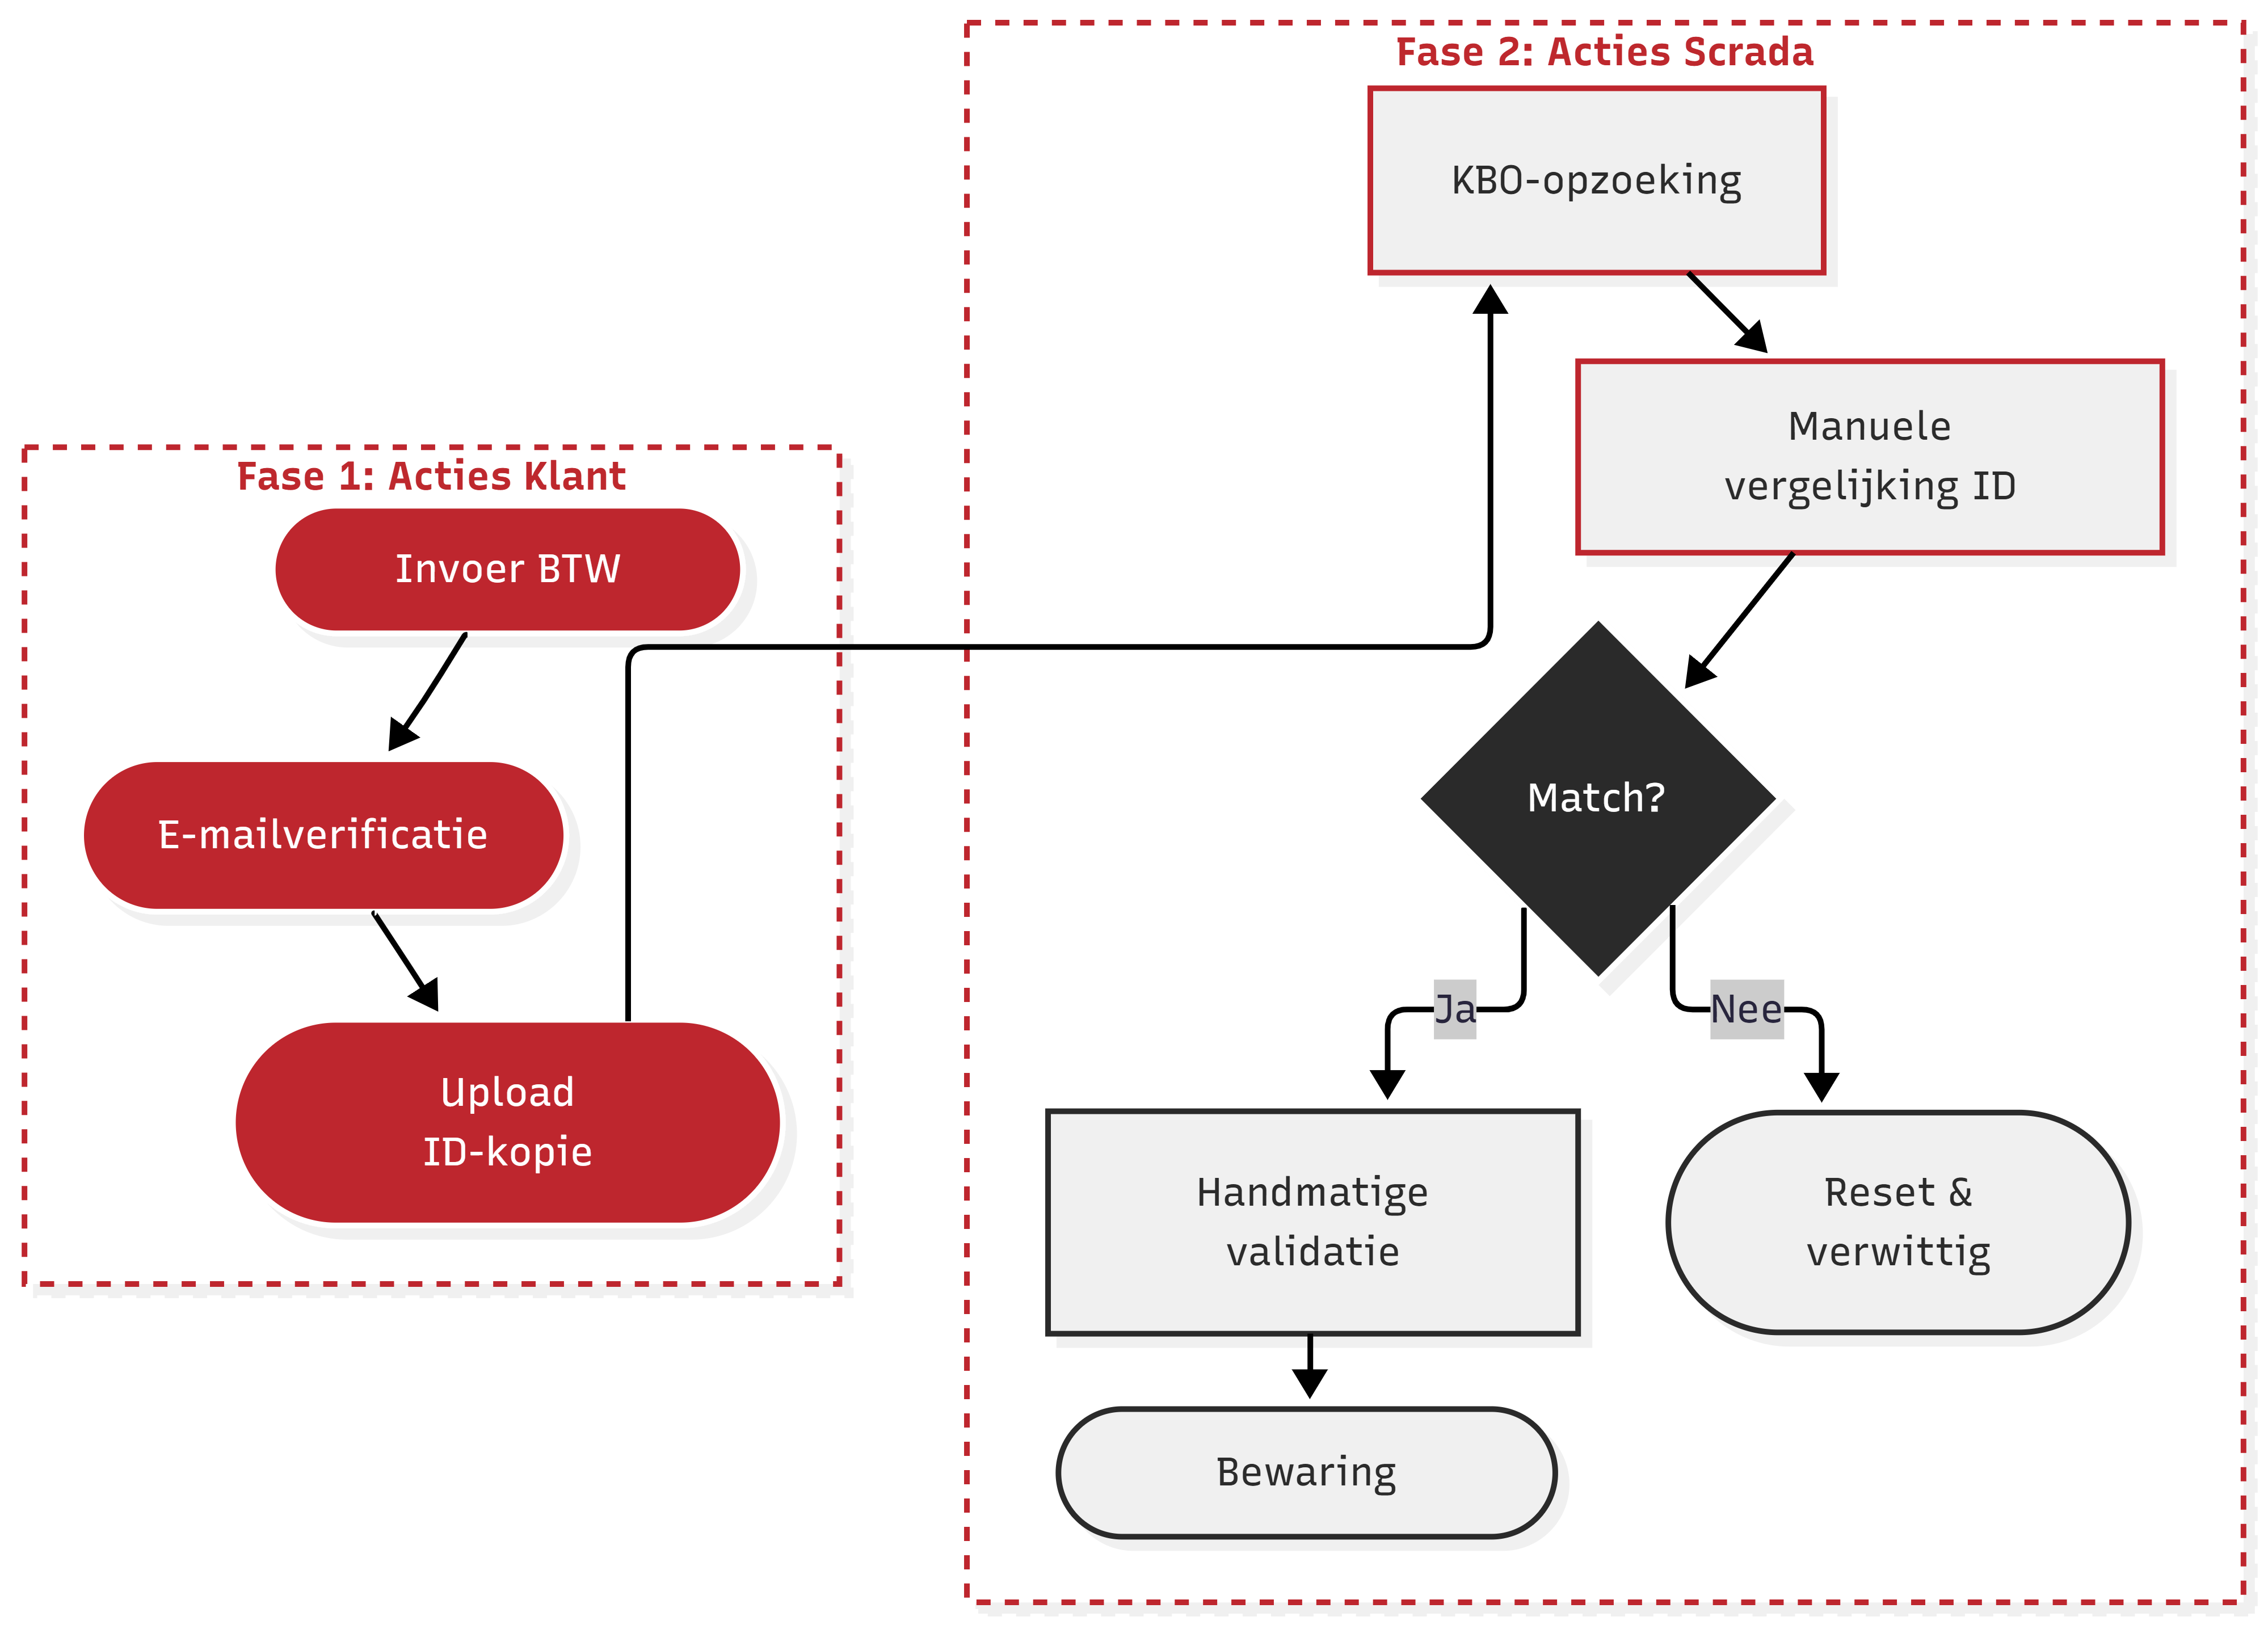
\includegraphics[width=\linewidth, keepaspectratio]{as_is.png}
        \captionof{figure}{\small AS-IS: Huidig manueel proces}
    \end{minipage}
    \hfill
    \begin{minipage}[t]{0.49\linewidth}
        \centering
        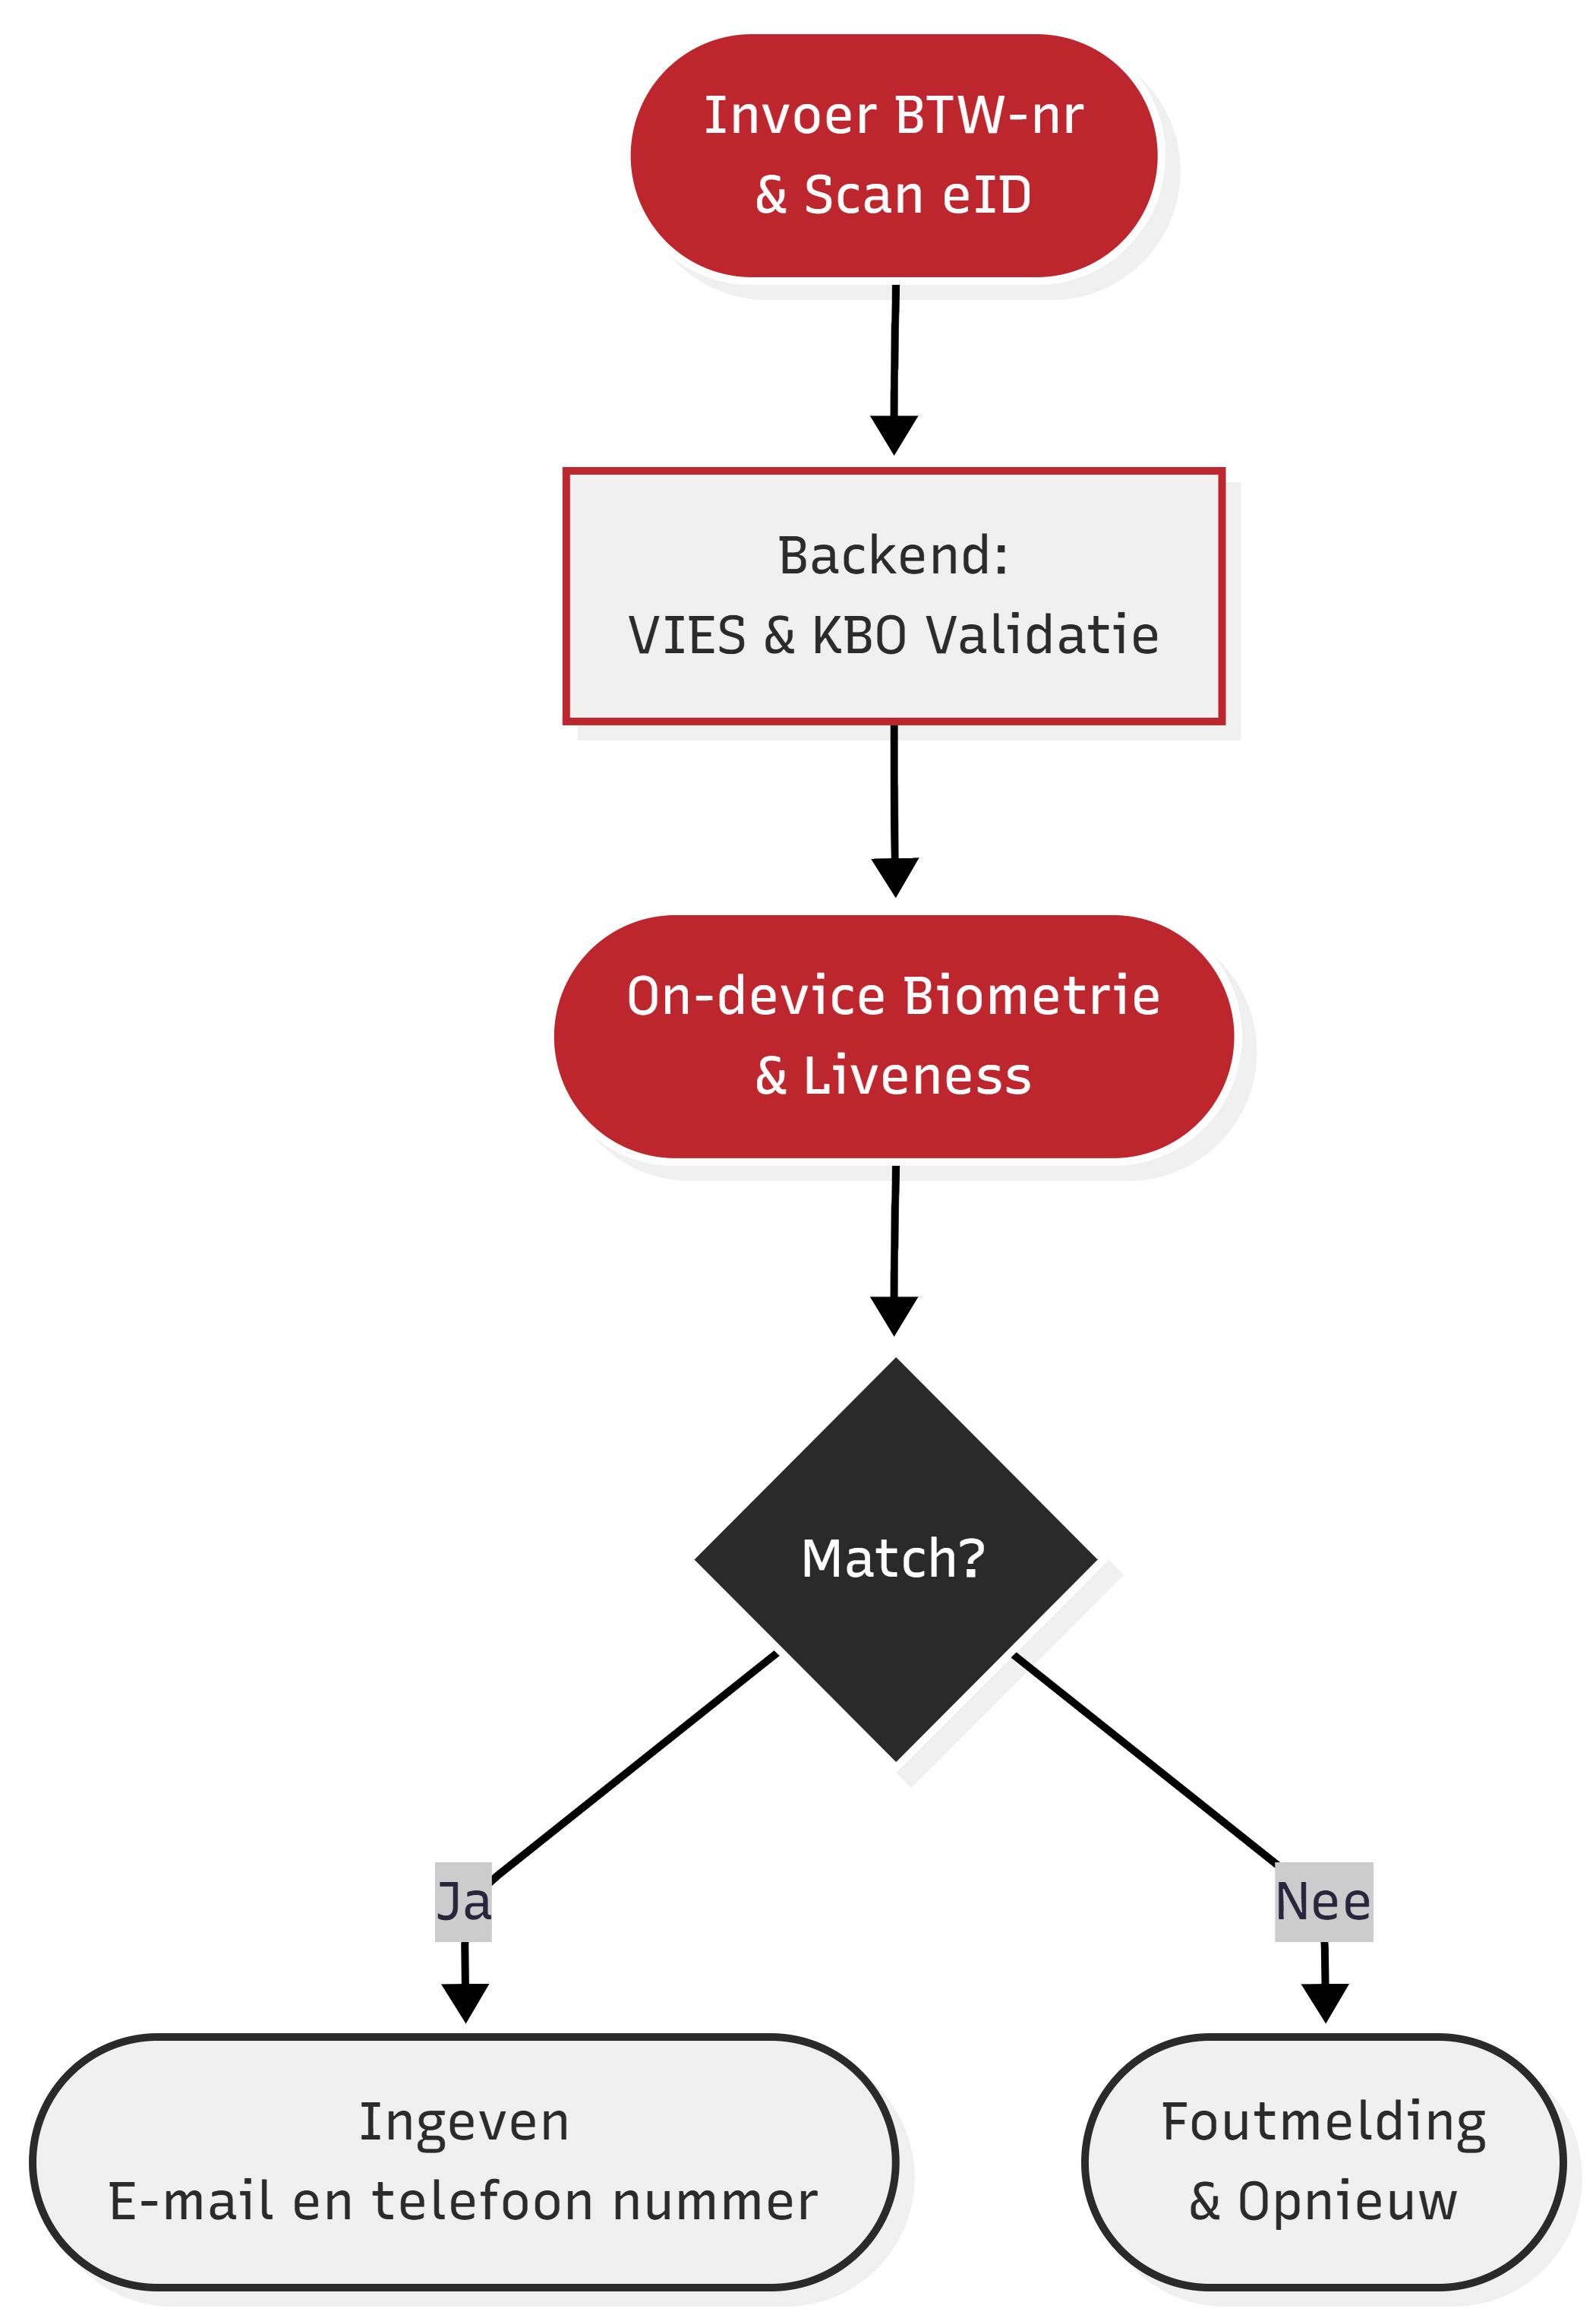
\includegraphics[width=\linewidth, keepaspectratio]{to_be.png}
        \captionof{figure}{\small TO-BE: Geautomatiseerde flow}
    \end{minipage}
\end{center}
\end{posterbox}

\columnbreak

\begin{posterbox}{\faProjectDiagram \quad Systeemarchitectuur}
De architectuur heeft een ontkoppeling tussen de lokale identiteitsverwerking (Flutter) en de centrale validatie \& logica (.NET). Dit garandeert Privacy-by-Design: 
biometrische data wordt enkel lokaal verwerkt en nooit centraal opgeslagen.
\vspace{0.4cm}
\begin{center}
    \begin{minipage}[t]{0.45\linewidth}
        \centering
        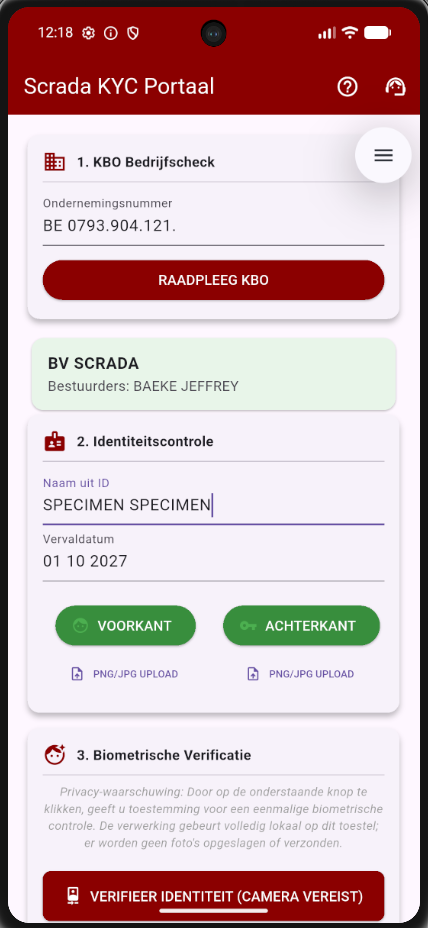
\includegraphics[width=0.7\linewidth]{poster-screenshot.png}
    \end{minipage}%
    \hfill
    \begin{minipage}[t]{0.45\linewidth}
        \centering
        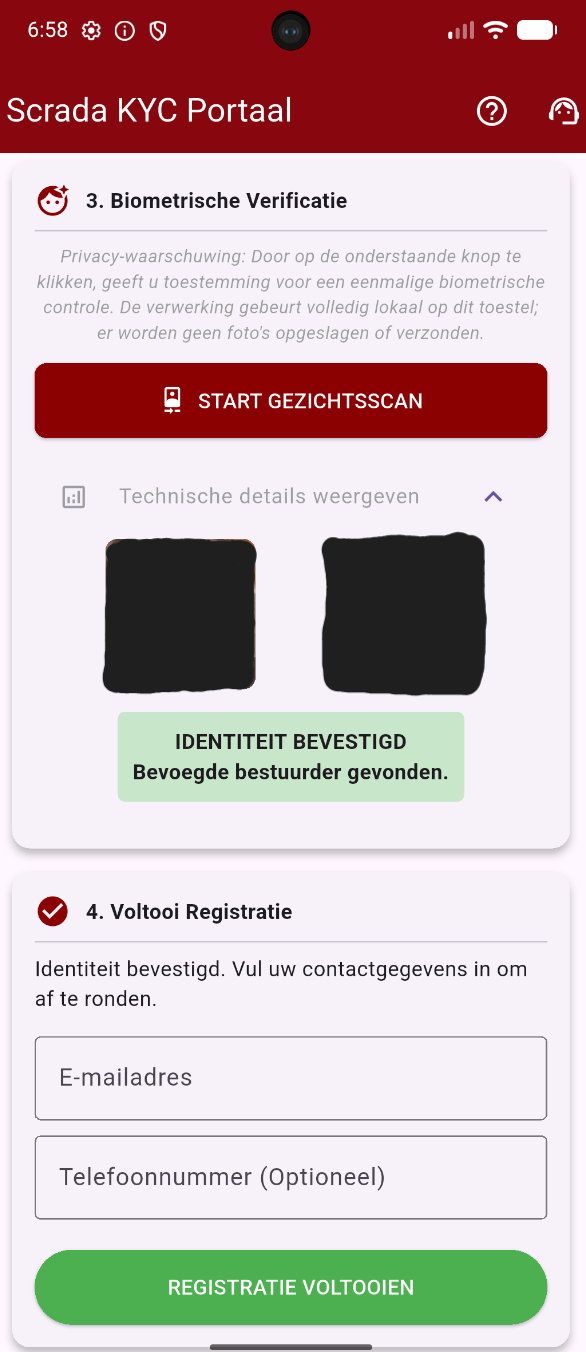
\includegraphics[width=0.7\linewidth]{biometrics_poster.png}
    \end{minipage}\\[0.2cm]
    \captionof{figure}{\small Data-flow \& Biometrie}
\end{center}
\end{posterbox}

\begin{posterbox}{\faCheckDouble \quad Resultaten \& Verificatie}
De PoC bewijst dat een volledige check maar ongeveer 3 minuten duurt. 
\vspace{0.5cm}
\begin{center}
\renewcommand{\arraystretch}{1.5}
\begin{tabular}{|l|l|l|l|}
    \hline
    \textbf{\textcolor{hogent-blue}{Scenario}} & \textbf{\textcolor{hogent-blue}{Input Type}} & \textbf{\textcolor{hogent-blue}{Score}} & \textbf{\textcolor{hogent-blue}{Resultaat}} \\ \hline
    Goede belichting & ID + Selfie & 80,4\% & Match (OK) \\ \hline
    Matige belichting & ID + Selfie & 64,0\% & Match (OK) \\ \hline
    Mismatch & ID + Andere persoon & -6,1\% & No Match \\ \hline
    Spoofing (Foto) & ID + Foto & N.v.t. & Liveness Failed \\ \hline
\end{tabular}
\end{center}
\end{posterbox}

\begin{posterbox}{\faFlagCheckered \quad Conclusie \& Reflectie}
\begin{itemize}
    \item \textbf{Impact:} KYC-proces volledig geautomatiseerd \& doorlooptijd gereduceerd met ca. 70\%.
    \item \textbf{Resultaat:} Een efficiënte, fraudeveilige en GDPR-conforme onboarding voor Scrada.
    \item \textbf{Toekomst:} Integratie van officiële KBO-API en NFC-authenticatie voor maximale betrouwbaarheid.
\end{itemize}
\end{posterbox}

\end{multicols}
\end{document}